\documentclass{article}

\usepackage[margin=2cm]{geometry}

%        UK date        %
\usepackage{datetime}
\newdateformat{UKvardate}{%
\THEDAY\ \monthname[\THEMONTH] \THEYEAR}
\UKvardate

\usepackage{hyperref}
\usepackage{subcaption}
\usepackage{todonotes}
\newcommand{\itodo}[1]{\todo[inline]{#1}}

% refcheck highlights labels and checks for unused labels
% \usepackage{refcheck}

\usepackage{tabularx}
\newcolumntype{C}{>{\centering\arraybackslash}X}
\setlength{\extrarowheight}{7pt}

\usepackage{mathtools}
\usepackage{amsmath}
\usepackage{amssymb}
\usepackage{amsthm}
\newtheorem{theorem}{Theorem}
\newtheorem{lemma}[theorem]{Lemma}

\theoremstyle{definition}
\newtheorem{definition}[theorem]{Definition}

\theoremstyle{remark}
\newtheorem*{example}{Example}
\newtheorem*{remark}{Remark}

% suppress full stop after last number
\usepackage{etoolbox}
\makeatletter
\patchcmd{\@thm}{\thm@headpunct{.}}{\thm@headpunct{}}{}{}
\makeatother

\usepackage{bbm}
\newcommand{\bb}[1]{\mathbb{#1}}
\newcommand{\cl}[1]{\mathcal{#1}}
\newcommand{\bl}[1]{\mathbf{#1}}
\newcommand{\fr}[1]{\mathfrak{#1}}

\DeclarePairedDelimiterXPP{\abs}[1]{}{\lvert}{\rvert}{}{{#1}}
\DeclarePairedDelimiterXPP{\norm}[2]{}{\lVert}{\rVert}{_{#2}}{#1}
\DeclarePairedDelimiterXPP{\inner}[3]{}{\langle}{\rangle}{_{#3}}{#1, #2}

\DeclareMathOperator*{\argmax}{arg\,max}
\DeclareMathOperator*{\argmin}{arg\,min}

\newcommand{\set}[1]{\left\{#1\right\}}
\newcommand{\pipeset}[2]{\left\{#1\mid#2\right\}}
\newcommand{\textset}[2]{\pipeset{#1}{\text{#2}}}

\usepackage{interval}
\intervalconfig{soft open fences}

\newcommand{\col}[1]{\mathop{}\!\mathrm{col}\left(#1\right)}
\newcommand{\row}[1]{\mathop{}\!\mathrm{row}\left(#1\right)}
\newcommand{\rnk}[1]{\mathop{}\!\mathrm{rank}\left(#1\right)}
\newcommand{\knl}[1]{\mathop{}\!\mathrm{ker}\left(#1\right)}
\newcommand{\rng}[1]{\mathop{}\!\mathrm{range}\left(#1\right)}
\newcommand{\diag}[1]{\mathop{}\!\mathrm{diag}\left(#1\right)}
\newcommand{\lspan}[1]{\mathop{}\!\mathrm{span}\left(#1\right)}
\newcommand{\trace}[1]{\mathop{}\!\mathrm{tr}\left(#1\right)}
\newcommand{\id}[1]{\mathop{}\!\mathrm{id}_{#1}}
\newcommand{\cond}[1]{\mathop{}\!\mathrm{cond}\left(#1\right)}
\newcommand{\vect}[1]{\mathop{}\!\mathrm{vec}\left(#1\right)}

\newcommand{\pd}{\mathop{}\!\partial}
\newcommand{\di}[1]{\mathop{}\!\mathrm{d}{#1}}
\newcommand{\iu}{{i\mkern1mu}}

\newcommand{\restrict}[2]{{\left.\kern-\nulldelimiterspace#1\vphantom{|}\right|_{#2}}}

\newcommand{\wto}{\rightharpoonup}

\usepackage[algoruled, noline, linesnumbered, noend]{algorithm2e}

\usepackage{tikz}
\usepackage{pgfplots}
\pgfplotsset{compat=1.18}


\usepackage[backend=biber, url=false, isbn=false, maxbibnames=99, giveninits=true, date=year]{biblatex}
% \renewbibmacro{in:}{}
\addbibresource{refs.bib}

%        Custom enumerations        %
\usepackage{enumitem}


\title{Motion Detection as a Consequence of Foreground/Background Separation using QR Streaming Dynamic Mode Decomposition}
\author{Peter Oehme\thanks{EPFL, Lausanne, Switzerland (\href{mailto:peter.oehme@epfl.ch}{peter.oehme@epfl.ch})}}

\begin{document}
    \maketitle

    \begin{abstract}
        This report discusses a QR compressed streaming DMD algorithm with applications to motion detection and foreground/background separation in real-time data-based video processing without full data availability. We explain how the iterative updating works hand in hand with the data compression to handle individually provided data and adaptively select relevant information within the video frames. Further, we indicate how a basic foreground/background separation algorithm directly yields a motion detection method in the streaming data setting, and how it can be adapted to serve its original purpose of foreground object detection. Three different realistic datasets are employed to demonstrate the efficacy of this approach, and to demonstrate its short-comings in noise resistance and background permanence.
    \end{abstract}

    \section{Introduction}

    The Dynamic Mode Decomposition (DMD) currently enjoys a lot of attention for applications in data-driven settings due to its versatility. Most of these applications use the fact that DMD does not require any knowledge of the data to obtain generalised image processing systems (\cite{Grosek2014, Kutz2015, Bi2018, Erichson2019a, UlHaq2020}). Among these image processing problems we tackle the tasks of foreground/background separation, and, due to the details of our implementation, motion detection. We demonstrate that our algorithms produce usable and reproducable results in a real-time viable runtime through the means of a streaming DMD implementation.

    The two main aspects of streaming DMD are: the compression of the data, and the use of the streaming framework, where the algorithm operates on iteratively supplied data snapshots. The former of these two has made advances through the use of compressed sensing as well as randomised sampling methods, see e.g.~\cite{Brunton2016a} and~\cite{Erichson2019}; however, the compression heavily depends on how well one can approximate currently available data, and most update computations are expensive. To remedy the update costs, a streaming DMD and an online DMD have been developped by~\cite{Hemati2014} and~\cite{Nedzhibov2023}. Here, the authors successively update approximates of the discretised Koopman operator by updating either projection matrices or the underlying SVD directly. This report aims to lay out a third option to these two publications, one that does not change the main DMD algorithm, but instead uses update formulae of the QR decomposition and the SVD to keep track of the necessary quantities for which we compute the DMD as motivated by the examination of snapshot reconstruction in~\cite{Drmac2020VandermondeKhatriRao}.

    We structure this report as follows: Section~\ref{sec:dmd} introduces the DMD and its accompanying quantities related to snapshot reconstruction and dynamic mode residuals. We also explain how simple QR compression works, and how it speeds up the evaluation of both the residuals and the reconstruction coefficients, concluding in an explanation of how to use update formulas to use QR decompression in an incremental algorithm. In Section~\ref{sec:motion-detection} we highlight how foreground/background separation works once one has computed the DMD of data matrices. By analysis of our streaming and compressed algorithm we explain how the dynamically reconstructed backgrounds suit themselves to motion detection, and we provide a way to take some of these dynamic backgrounds to perform the original separation task instead of motion detection. We demonstrate the performance of our basic Python implementation on three sample datasets in Section~\ref{sec:numerical-experiments}, and conclude the report in Section~\ref{sec:conclusion} by pointing out various ways of further research to improve the results presented here.
    
    \section{Dynamic Mode Decomposition}\label{sec:dmd}

As a crucial, data-agnostic method for this report we use the \emph{Dynamic Mode Decomposition} (DMD). DMD is a data-agnostic computational tool founded on Koopman operator theory~\cite{Rowley2009, Williams2015}. For a discrete dynamical system
\begin{equation*}
    x_{k + 1} = K x_k,
\end{equation*}
where $K$ is an unknown linear operator, DMD uses an algorithm such as Algorithm~\ref{alg:schmid-dmd} to compute approximate eigenpairs known as dynamic modes and dynamic amplitudes, or Ritz pairs, of $K$ from a sequence of data snapshots ${(\bl{f}_k)}_{k = 1}^M, M \in \bb{N}$, split into two data matrices $\bl{X} = (\bl{f}_1, \bl{f}_2, \dots, \bl{f}_{M - 1})$ and $\bl{Y} = (\bl{f}_2, \bl{f}_3, \dots, \bl{f}_M)$, by computing Galerkin approximations of the original matrix. Afterwards, we can use the dynamic pairs to compute reconstructions of the original data and make predictions for future points in time based on these reconstruction.

\begin{algorithm}[!ht]
    \caption{Schmid DMD, introduced in~\cite{Schmid2010}}\label{alg:schmid-dmd}
    \KwData{Data matrices $\bl{X}, \bl{Y} \in \bb{C}^{N \times M}$, an optional tolerance $\tau > 0$}
    Compute the SVD $\bl{X} = U \Sigma V^*$, truncate the SVD to dimension $R$ for a given tolerance $\tau$\;
    Define the approximate $\tilde{K} = U^* \bl{Y} V \Sigma^{-1} \in \bb{C}^{R \times R}$\;
    Determine $R$ eigenpairs $(\lambda_i, w_i), i = 1, 2, \dots, R$\;
    Set $W = (w_1, w_2, \dots, w_R)$\;
    \Return{Ritz values $\lambda_1, \lambda_2, \dots, \lambda_R$ and Ritz vectors $U W$}
\end{algorithm}

Unfortunately, not all dynamic modes are good approximations of $K$'s eigenvalues on the data matrices $\bl{X}$ and $\bl{Y}$. To get a feeling for how well each DMD mode can approximate an eigenpair of $K$ we consider the \emph{data-driven Ritz residuals} of the dynamic modes $Z = U W$ defined in~\cite{Drmac2020} as follows:
\begin{equation}\label{eq:residual}
    r_i \coloneqq \norm{K (U w_i) - \lambda_i U w_i}{2} = \norm{(\bl{Y} V \Sigma^{-1}) w_i - \lambda_i z_i}{2}.
\end{equation}
We use these residuals not only to check for the suitability as eigenpairs, but they can also give us an indication for other properties we shall discuss in Section~\ref{sec:motion-detection}.

After selecting a subset $\cl{I} \subseteq \set{1, 2, \dots, R}$ with $\ell \in \bb{N}$ indices of the available dynamic modes we want to reconstruct the known data from these modes. This is equivalent to solving the problem
\begin{equation*}
    \min\limits_{\alpha \in \bb{C}^\ell} \sum\limits_{i = 1}^{M - 1} \omega_i \norm*{\bl{f}_i^2 - \sum\limits_{j = 1}^\ell \alpha_{\cl{I}_j} \lambda_{\cl{I}_j}^{i - 1} z_{\cl{I}_j}}{2}^2 = \min\limits_{\alpha \in \bb{C}^\ell} \norm{(\bl{X} - Z \diag{\alpha} \bb{V}(\lambda)) W}{F}^2
\end{equation*}
as defined in~\cite[Equation~(3.1)]{Drmac2020VandermondeKhatriRao}, where $\bb{V}(\lambda) \in \bb{C}^{\ell \times M - 1}$ is the Vandermonde matrix of the dynamic amplitudes and $\omega_i \in \bb{C}$ are given weights. Following the argument in~\cite{Drmac2020VandermondeKhatriRao}, the solution to this least squares problem is given by
\begin{equation}\label{eq:coefficients}
    \alpha = {\left( (Z^* Z) \odot (\overline{\bb{V}(\lambda) W^2 \bb{V}^*(\lambda)}) \right)}^{-1} \left( \overline{\bb{V}(\lambda) W} \odot (Z^* \bl{X} W) e \right),
\end{equation}
where $e$ is the vector containing only ones, and $\odot$ denotes the Hadamard product of matrices. Finally, we define the reconstruction of a snapshot at time $k$ as the combination of this parameter vector with the other, previously computed quantities:
\begin{equation}\label{eq:reconstruction}
    \bl{x}_\text{re}(k) \coloneqq \sum\limits_{i = 1}^\ell \alpha_{\cl{I}_i} \lambda_{\cl{I}_i}^{k - 1} z_{\cl{I}_i}.
\end{equation}
We will use this reconstruction formula repeatedly and for different ways of computing the coefficients $\alpha$ for the same input data. Most importantly we note that by splitting the indices over which we sum further into two sets $\cl{I}_1$ and $\cl{I}_2$, we obtain a decomposition $\bl{x}_\text{re} = \bl{x}_\text{re}^{(1)} + \bl{x}_\text{re}^{(2)}$, which we will use in Section~\ref{sec:motion-detection} after consideration of a proper splitting method.

\subsection{QR Compressed DMD}\label{subsec:qr-compression} % MARK: QR COMPRESSION

Another option of getting around the prohibitively large dimension $N$ is to compress the data before computing any DMD quantities. There exist multiple frameworks for these compressions, such as Compressive Sensing~\cite{Brunton2016a}, QR Compression~\cite{Drmac2020VandermondeKhatriRao}, and Randomised Sampling~\cite{Erichson2019}. In this report we choose compression by means of the QR decomposition $Q R = (\bl{f}_1, \bl{f}_2, \dots, \bl{f}_M)$. As a consequence, we introduce two layers of abstraction: the uncompressed and the compressed. We can classify the general steps of algorithms relying on DMD as belonging to one of these layers as follows:
\begin{enumerate}
    \item In the uncompressed layer we first have to compress the data $(\bl{f}_1, \bl{f}_2, \dots, \cl{f}_M) = Q R$,
    \item then we perform DMD on the compressed data obtained from the columns of $R$, and
    \item lastly we project reconstructions and DMD modes back up into the uncompressed layer for analysis and further treatment as part of our general data processing objective.
\end{enumerate}
Most of the previous quatities can be computed in the compressed domain, thus allowing for more efficient computation overall if we do not require any access to the full dimensional quantities.

Importantly, we can compute the residuals of the dynamic pairs as
\begin{equation*}
    r_i = \norm{\bl{Y} V \Sigma^{-1} w_i - \lambda_i Q U w_i}{2} = \norm{Q R(\colon, 2 \colon M) V \Sigma^{-1} w_i - \lambda_i Q U w_i}{2} = \norm{R(\colon, 2 \colon M) V \Sigma^{-1} w_i - \lambda_i U w_i}{2},
\end{equation*}
assuming that we calculated $R = U \Sigma V$ instead of the SVD of the uncompressed data, as well as the coefficients of the reconstruction through the following expression
\begin{equation*}
    \alpha = {\left( (R^* R) \odot (\overline{\bb{V}(\lambda) W^2 \bb{V}^*(\lambda)}) \right)}^{-1} \left( \overline{\bb{V}(\lambda) W} \odot (R^* \bl{G} W) e \right),
\end{equation*}
where $\bl{G} = Q^* \bl{X}$ are the compressed  data snapshots, where the structure remains similar to the original problem in Equation~\eqref{eq:coefficients}. On the other hand, to obtain the uncompressed reconstructions and dynamic modes we always need to compute $Q \bl{f}_\text{re}$ or $Q z_i$, which is a disadvantage only if we need frequent access to the high-dimensional modes.

\subsection{QR Streaming DMD}\label{subsec:qr-update} % MARK: QR STREAMING

To our benefit, the QR decompression introduced in Subsection~\ref{subsec:qr-compression} can be easily updated to a streaming setting: Instead of having all data snapshots available at once, we get each $\bl{f}_k$ one by one. As such, it is necessary to devise a way to continuously update the compressed representation of our available data. We do this in two steps: First off all, it is necessary to add columns to the QR decomposition. This is generally useful in the streaming setting because we always assume to get more data, one at a time. Secondly, in the case of a limited snapshot memory we want to delete the first column of the present QR decomposition to save memory in the long run and to speed up the individual computations we might undertake in the compressed domain.

Adding a column to an already existing QR decomposition works as follows: Suppose your current data matrix is $\bl{X}_\text{old} = (\bl{f}_1, \bl{f}_2, \dots, \bl{k})$ and we now its QR decomposition $\bl{X}_\text{old} = Q R$. To compute the QR decomposition of the new data matrix $(\bl{X}_\text{old}, \bl{f}_{k + 1})$, we require the QR decomposition of the incoming data snapshot orthogonalised w.r.t.\ the previous QR basis
\begin{equation*}
    (\id{} - Q Q^*) \bl{f}_{k + 1} = \tilde{Q} \tilde{R}.
\end{equation*}
This allows us to write $\bl{X}_\text{new}$ as the updated QR Decomposition
\begin{equation*}
    \bl{X}_\text{new} = (Q, \tilde{Q}) \begin{pmatrix}
        R & Q^* \bl{f}_{k + 1} \\
        0 & \tilde{R}
    \end{pmatrix}.
\end{equation*}

Removing the first column, on the other hand, is a bit more involved. In this case, we desire to know the QR decomposition of $\bl{X}_\text{new} = (\bl{f}_2, \bl{f}_3, \dots, \bl{f}_k)$, whereas we a priori know only $Q R = \bl{X}_\text{old} = (\bl{f}_1, \bl{f}_2, \dots, \bl{f}_k)$. Simply removing the first column of $R$ is not sufficient because the new matrix $\tilde{R}$ would not be triangular, instead we observe the following sparsity pattern:
\begin{equation*}
    \tilde{R} = \begin{pmatrix}
        \times & \times & \dots & \times \\
        \times & \times & \dots & \times \\
         & \times & \dots & \times \\
         & & \ddots & \vdots \\
        \bl{0} & & & \times \\
    \end{pmatrix}
\end{equation*}
Thus, we need to rediagonalise this matrix. We use Givens or Householder rotations akin to~\cite{Daniel1976} and obtain a sequence $H_{k - 1} \dots H_2 H_1$ which, when applied to $\tilde{R}$ reduces it to upper triangular form. We gather the corresponding inverse rotations $H_1^* H_2^* \dots H_{k - 1}^*$ and multiply all of them before applying them to the $Q$ matrix, thus resulting in
\begin{equation*}
    Q \tilde{R} = \underbrace{Q (H_1^* H_2^* \dots H_{k - 1}^*)}_{\eqqcolon \hat{Q}} \underbrace{(H_{k - 1} \dots H_2 H_1) \tilde{R}}_{\eqqcolon \hat{R}}.
\end{equation*}
Finally, we are left with the new QR decomposition $\bl{X}_\text{new} = \hat{Q} \hat{R}$.

A prototype of a streaming DMD implementation for sequential data, that is $\bl{y}_k = \bl{x}_{k + 1}$, is given in Algorithm~\ref{alg:qr-streaming-dmd}. The parameter $\ell_\text{mem} \in \bb{N}$ represents the length of the snapshot memory $\fr{M}$, that is the maximum number of data snapshots stored throughout the runtime of the algorithm. Initially, we set the snapshot memory $\fr{M}$ as the empty set.

\begin{algorithm}[!ht]
    \caption{QR Streaming DMD}\label{alg:qr-streaming-dmd}
    \KwData{Incoming data $\bl{x}_k, \bl{y}_k \in \bb{C}^N$, the current memory $\fr{M}$, the maximal size of memory $\ell_\text{mem}$, an optional tolerance $\tau > 0$}
    \If{$\abs{\fr{M}} = 0$}{
        Set $\fr{M} = \set{\bl{x}_k}$\;
        Compute the QR decomposition $Q R = \texttt{qr}((\fr{M}, \bl{y}_k))$\;
        Compute the SVD $R(\colon, 1) = U \Sigma V^*$\;
    }
    \ElseIf{$\abs{\fr{M}} > 0$ and $\abs{\fr{M}} < \ell_\text{mem}$}{
        Append $\bl{x}_k$ to $\fr{M}$\;
        Update the QR decomposition by adding the column $\bl{y}_k$\;
        Update the SVD decomposition by adding the column $\bl{y}_k$\;
    }
    \Else{
        Append $\bl{x}_k$ to $\fr{M}$, remove the first element of $\fr{M}$\;
        Update the QR decomposition by adding the column $\bl{y}_k$ and removing the first colum\;
        Update the SVD decomposition by adding the column $\bl{y}_k$ and removing the first colum\;
    }
    \Return{Schmid DMD on $R(\colon, 1 \colon \abs{\fr{M}}), R(\colon, 2 \colon \text{end})$ with tolerance $\tau$, see Algorithm~\ref{alg:schmid-dmd}}
\end{algorithm}

\subsection{Updating the SVD} % MARK: SVD UPDATE

After every update of the QR decomposition, be it the addition of a column, the deletion of the first column, or both during a single iteration of the streaming algorithm, we are left with a new matrix $R$. During the QR compressed DMD algorithm, we would need to recalculate the SVD of this matrix after every update, however we can use similar updating procedures for the SVD. Suppose that we have previously computed the SVD $\bl{X}_\text{old} = U_\text{old} \Sigma_\text{old} V_\text{old}^* \in \bb{C}^{N \times k}$. The addition of a column begins with the following sequence of computations:
\begin{align*}
    \bl{X}_\text{new} &= (\bl{X}_\text{old}, 0) + \bl{f}_\text{new} e_{k + 1}^T \\
     &= U_\text{old} \Sigma_\text{old} (V_\text{old}^T, 0) + \bl{f}_\text{new} e_{k + 1}^T \\
     &= (U_\text{old}, \bl{f}_\text{new}) \begin{pmatrix}
        \Sigma_\text{old} & 0 \\
        0 & 1 \\
     \end{pmatrix} \begin{pmatrix}
        V_\text{old}^* & 0 \\
        0 & 1
     \end{pmatrix} \\
     &= (U_\text{old}, \bl{r}) \begin{pmatrix}
        \Sigma_\text{old} & \bl{d} \\
        0 & \rho \\
     \end{pmatrix} \begin{pmatrix}
        V_\text{old}^* & 0 \\
        0 & 1
     \end{pmatrix},
\end{align*}
where we used the following projected quantities:
\begin{equation*}
    \bl{d} \coloneqq U^* \bl{f}_\text{new},\quad \bl{p} \coloneqq (\id{} - U U^*) \bl{f}_\text{new},\quad \rho \coloneqq \norm{\bl{p}}{2},\quad \bl{r} = \bl{p} / \rho.
\end{equation*}
As a last step, it remains to compute the SVD of the central arrowhead matrix
\begin{equation*}
    \begin{pmatrix}
        \Sigma_\text{old} & \bl{d} \\
        0 & \rho \\
     \end{pmatrix} = \tilde{U} \tilde{\Sigma} \tilde{V}^*,
\end{equation*}
for which there exist efficient algorithms with a runtime of $\cl{O}((k + 1)^2)$, see e.g.~\cite{Gu1995, JakovcevicStor2015, Jiang2023}. Afterwards, we assemble the new SVD by multiplying
\begin{equation*}
    \bl{X}_\text{new} = ((U_\text{old}, \bl{r}) \tilde{U}) \tilde{\Sigma} \left( \tilde{V}^* \begin{pmatrix}
        V_\text{old}^* & 0 \\
        0 & 1
     \end{pmatrix} \right) = U_\text{new} \Sigma_\text{new} V_\text{new}^*.
\end{equation*}
Thus, whenever we add a row to the data matrix and update the corresponding QR decomposition, we can similarly update the underlying SVD for a faster computation.

The analogous removal of the first column also reduces to the computation of the eigendecomposition of a diagonal-plus-rank-one matrix, which for brevity we leave out of this report. If the reader is interested in these methods, we refer them to sources such as~\cite{Jiang2023}.

    \section{Foreground/Background Separation and Motion Detection}\label{sec:motion-detection}

In this section, we introduce an application of DMD in image processing. In particular, we link the Ritz values computed in Section~\ref{sec:dmd} to a segmentation of foreground and background data, and use these decompositions to compute a priori data-agnostic foreground masks. This approach was first introduced in~\cite{Grosek2014}, where the authors computed the DMD for a set of video frames and reconstructed one background snapshot to compute a foreground mask for every frame. This paper relies on the full decomposition, making it slow when compared to different compressed approaches such as compressive DMD or randomised DMD.

\subsection{Foreground/Background Separation}\label{subsec:fg-bg-separation} % MARK: FB/BG

The main idea used in~\cite{Grosek2014, Kutz2015, Erichson2016} is to compare the logarithmic dynamic amplitudes
\begin{equation*}
    \omega_i = \log{(\lambda_i)},\quad i = 1, 2, \dots, R,
\end{equation*}
and find those pairs for which the logarithmic amplitude is close to zero. These Ritz values change very slowly during each successive time step in the reconstruction~\ref{eq:reconstruction}, hence it is suitable to consider these as the background of the data. Setting $\cl{I}_\text{BG} \subseteq \set{1, 2, \dots, R}$ as the subset of these background amplitudes we can split the reconstruction formula into a foreground and a background object as follows
\begin{equation*}
    \bl{f}_\text{re}(k) = \bl{f}_\text{BG}(k) + \bl{f}_\text{FG}(k) = \sum\limits_{i \in \cl{I}_\text{BG}} \alpha_i \lambda_i^{k - 1} z_i + \sum\limits_{i \not\in \cl{I}_\text{BG}} \alpha_i \lambda_i^{k - 1} z_i.
\end{equation*}
Lastly, we define the foregound mask as the thresholded matrix-valued function
\begin{equation*}
    \left(m_\text{FG}(k)\right)_{i, j} \coloneqq \begin{cases}
        1, & \abs{\bl{f}_k - \bl{f}_\text{BG}(k)} \geq \tau \\
        0, & \abs{\bl{f}_k - \bl{f}_\text{BG}(k)} < \tau
    \end{cases},
\end{equation*}
where $\tau > 0$ is a tolerance chosen prior to the computation.

\subsection{Backgrounds in QR Streaming DMD} % MARK: MOTION

The procedure described in Subsection~\ref{subsec:fg-bg-separation} illustrates the application of the DMD method to imaging problems, given that we know the entirety of the data matrix beforehand. This assumption may not be valid in cases where storing large amounts of data is impractical or the data are not available all at once. In such a case it is convenient to employ a streaming framework and iteratively compute the desired results.

There is, however, one immediate problem: If we constrain the size of the memory available during the computation, we might encounter the case that all relevant data of the actual background does no longer appear in the kept memory. Consider, for example, a streaming implementation with a memory of exactly $10$ snapshots. Suppose that $\bl{f}_T$ contains only the background, and that every snapshot after it has some moving object in it. Then, after advancing $10$ steps in time, the memory of the method is $\set{\bl{f}_{T + 1}, \bl{f}_{T + 2}, \dots, \bl{f}_{T + 10}}$, and therefore no longer contains any pure representation of the original background. Thus, a comparison of the streaming background with the incoming data yields a foreground mask only containing local and recent changes: that is if some object moves within a few frames of the video, then we can detect changes in its position. Effectively, this method only allows for detection of a \emph{motion mask} instead of complete foreground/background separation, where the motion is identified as the change with respect to the background recovered from the most recent streaming data. A side effect of this analysis is that large moving objects with a uniform texture will register in the motion mask only along the moving edges, e.g.\ the front and the back of a moving bicycle. We illustrate this behaviour more in Section~\ref{sec:numerical-experiments}.

To mitigate the lack of a fixed reference background for streaming applications with limited available memory, we can try and compute a more permanent background by evaluating the approximation quality of the current DMD residuals as defined in Equation~\ref{eq:residual}. Looking at the minimum absolute value of the residuals from the numerical example in Subsection~\ref{subsec:pedestrians}, we notice that at some points in time the value increases significantly, whereas before it remained about constant, see Figure~\ref{fig:pedestrian-residual}. We exploit this by updating the stored background reconstruction whenever the minimal residual is below a certain predefined tolerance $\rho > 0$. Whenever this threshold is exceeded, we compute the foreground mask of the current frame from the difference $\bl{f}_k - \bl{f}_\text{BG}$, where $\bl{f}_\text{BG}$ is the most recent background reconstruction with a minimal residual smaller than the tolerance. This has the additional benefit that we do not compute a foreground mask for pure background snapshots, hence reducing the output of the algorithm to actual time periods of interest, that is spans of time in which foreground objects move.

\begin{figure}[!ht]
    \centering
    \begin{tikzpicture}
        \pgfplotsset{
            width=16cm,
            height=7cm
        }
        \begin{axis}[
            xmin=0, xmax=846,
            ymin=1e-3, ymax=1e-1,
            ymode=log,
            xlabel={Index $i$},
            ylabel={Residual $r_i$}
        ]
            \addplot[smooth, thick, samples=50] coordinates {(50, 1e-1) (50, 1e-3)};
            \addplot[smooth, thick, samples=50] coordinates {(465, 1e-1) (465, 1e-3)};
            \addplot[smooth, thick, samples=50] coordinates {(575, 1e-1) (575, 1e-3)};
            \addplot[smooth, thick, samples=50] coordinates {(805, 1e-1) (805, 1e-3)};
            \addplot[fill=lightgray, draw=none] coordinates {(0, 1e-3) (50, 1e-3) (50, 1e-1) (0, 1e-1)} \closedcycle;
            \addplot[fill=lightgray, draw=none] coordinates {(465, 1e-3) (575, 1e-3) (575, 1e-1) (465, 1e-1)} \closedcycle;
            \addplot[fill=lightgray, draw=none] coordinates {(805, 1e-3) (846, 1e-3) (846, 1e-1) (805, 1e-1)} \closedcycle;
            \addplot[color=red, smooth, thick] table[col sep=comma, header=has colnames, x index={0}, y index={1}] {pedestrian_motion_res.csv};
        \end{axis}
    \end{tikzpicture}
    \caption{Residuals $r_i$ for the pedestrian dataset from Subsection~\ref{subsec:pedestrians} for a memory size of $5$ data snapshots; Red: residuals as computed during the streaming algorithm; Grey shaded areas indicate indices of frames where the algorithm determined the residual to be less than the specified tolerance $\rho$.}\label{fig:pedestrian-residual}
\end{figure}

This method has the benefit that backgrounds can change continually throughout the stream of data snapshots, and after a short readjustment period a relevant background will be computed. In contrast, a non-streaming DMD method relies entirely on the accuracy of the background prediction from all data at once, and may be substantially worse. Thus, using sets of data limited in time not only speeds up every single evaluation and allows for real-time applications, but it may also provide a more stable method.

    \section{Numerical Experiments}\label{sec:numerical-experiments}

Throughout this section we present some numerical experiments. These were selected from the \href{changedetection.net}{changedetection.net} datasets. Our procedure works as follows: While reading the data stream of images we normalise every image vector by its norm, such that $\norm{\bl{f}_k}{2} = 1$ holds for all input data. This data normalisation is useful in DMD because the scaling of the data directly influences the numerical computations and thus the quality of the returned quantities~\cite{Drmac2020}. Afterwards, we perform QR compressed streaming DMD as explained in Algorithm~\ref{alg:qr-streaming-dmd} on the incoming data. In a first run we plot the minimal values of all dynamic residuals for a small number of data snapshots to decide upon a cut-off tolerance for background and motion detection. Once this threshold has been chosen, we compute the background reconstructions and foreground masks as explained in Section~\ref{sec:motion-detection}. We repeat this process for a select number of parameter combinations, mostly varying the size of the data memory $\ell_\text{mem}$. Our experiments show that in the streaming setting, even a small number of stored snapshots and a low reconstruction/truncation rank suffice to provide good foreground masks.

All code used to generate the results of this report have been uploaded to \href{https://github.com/peoe/dmd-math-656/}{github.com/peoe/dmd-math-656/}. Included in this repository are a setup file for the Python environment required, as well as a script to aid in acquiring the relevant datasets.

\subsection{Detection of Pedestrians}\label{subsec:pedestrians} % MARK: PEDESTRIANS

The pedestrian dataset obtained from \href{changedetection.net}{changedetection.net} shows a section of a street with pedestrians and a bicyclist passing along the road. This example is a nice benchmark problem because the video contains both a stationary and not very noisy background, but it also includes different movement speeds.

We run both the motion detection and the foreground/background separation algorithm in the streaming DMD setting with a limited snapshot memory size of $\ell_\text{mem} \in \set{5, 10, 15, 20}$. For the foreground/background separation we consider the minimal residuals of the first $100$ frames to determine the residual tolerance $\rho > 0$, see Figure~\ref{fig:pedestrian-exp-residual} for a plot of these first residuals. Afterwards, we compute the separated foreground data with tolerances of $\rho \in \set{8 \cdot 10^{-3}, 5 \cdot 10^{-3}, 3 \cdot 10^{-3}, 10^{-3}}$ for the respective $\ell_\text{mem}$ snapshot memory size. We can see that the minimal residual for every memory size decreases initially as the memory slowly gets filled with snapshots. Then we enter a plateau phase where the minimal residual remains consistently small before increasing after $i = 50$ where the first pedestrian enters the frame. Noticably, the minimal residual for larger memory sizes spikes to a large number as soon as the scene changes upon the entrance of a moving foreground object. This is due to the fact that at this point the snapshot memory contains a larger number of snapshots does not contain the pedestrian, and hence the dynamic modes mostly reconstruct the static background instead of the moving foreground. This can be mitigated by choosing either a smaller memory size $\ell_\text{mem}$, or by dynamically reducing the length of the memory once we detect a spike in the minimal residual.

\begin{figure}[!ht]
    \centering
    \begin{tikzpicture}
        \pgfplotsset{
            width=16cm,
            height=7cm
        }
        \begin{axis}[
            xmin=0, xmax=100,
            ymin=1e-4, ymax=1e0,
            ymode=log,
            xlabel={Index $i$},
            ylabel={Residual $r_i$},
            legend style={
                at={(0.975, 0.05)},
                anchor=south east,
                legend columns=1,
            }
        ]
            \addplot[color=red, smooth, thick] table[col sep=comma, header=has colnames, x index={0}, y index={1}] {pedestrian_motion_res.csv}; \addlegendentry{$\ell_\text{mem} = 5$}
            \addplot[color=blue, smooth, thick] table[col sep=comma, header=has colnames, x index={0}, y index={2}] {pedestrian_motion_res.csv}; \addlegendentry{$\ell_\text{mem} = 10$}
            \addplot[color=orange, smooth, thick] table[col sep=comma, header=has colnames, x index={0}, y index={3}] {pedestrian_motion_res.csv}; \addlegendentry{$\ell_\text{mem} = 15$}
            \addplot[color=black, smooth, thick] table[col sep=comma, header=has colnames, x index={0}, y index={4}] {pedestrian_motion_res.csv}; \addlegendentry{$\ell_\text{mem} = 20$}
        \end{axis}
    \end{tikzpicture}
    \caption{Residuals $r_i$ for the pedestrian dataset for memory sizes $\ell_\text{mem} \in \set{5, 10, 15, 20}$; In colour: residuals as computed during the streaming algorithm.}\label{fig:pedestrian-exp-residual}
\end{figure}

For selecting the motion or foreground masks we determine an error threshold and select all pixels for which the dynamic background differs from the incoming data by more than the threshold. A comparison of the true image, the computed motion mask, and the foreground mask at frame number $100$ can be seen in Figure~\ref{fig:pedestrian-frame-100}. Notice that the motion mask highlights only the outline of the pedestrian --- as described above this occurs because the dynamic backgrounds in the motion detection procedure only store local information, and thus only detect the movement along object and texture boundaries.

\begin{figure}[!ht]
    \centering
    \begin{subfigure}{.3\textwidth}
        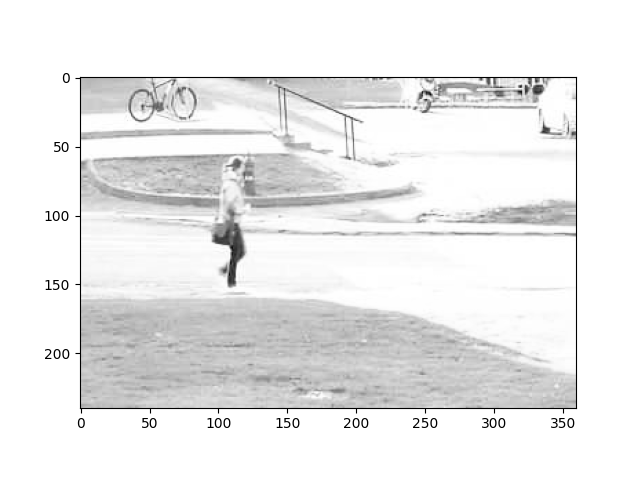
\includegraphics[width=\textwidth]{pedestrian_frame_100.png}
        \caption{True image}
    \end{subfigure}
    \hfill
    \begin{subfigure}{.3\textwidth}
        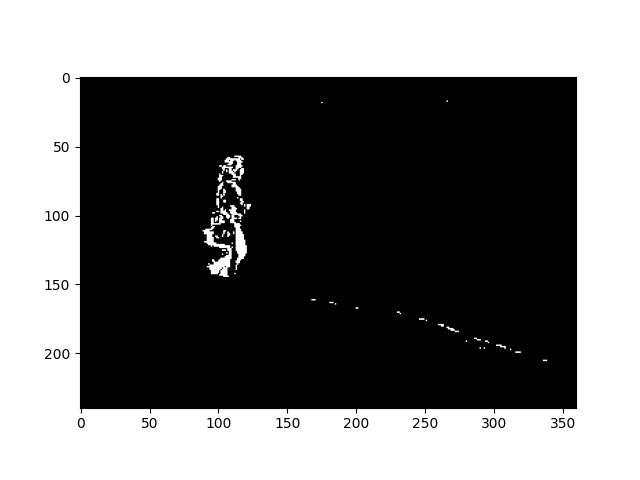
\includegraphics[width=\textwidth]{pedestrian_motion_frame_100.png}
        \caption{Motion mask}
    \end{subfigure}
    \hfill
    \begin{subfigure}{.3\textwidth}
        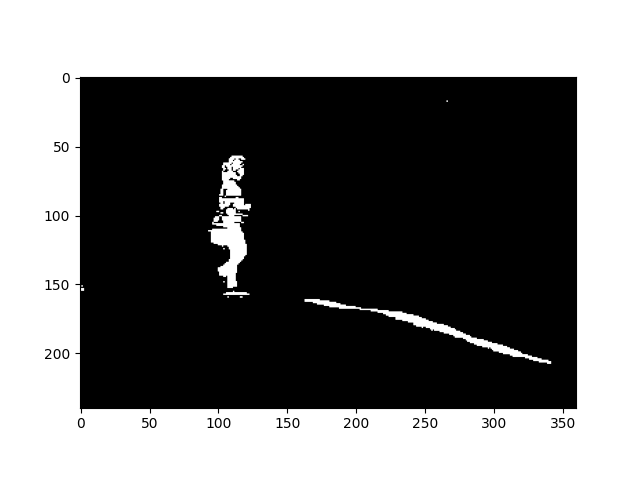
\includegraphics[width=\textwidth]{pedestrian_fg_frame_100.png}
        \caption{Foreground mask}
    \end{subfigure}
    \caption{Comparison of the true image, the motion mask, and the foreground mask for the pedestrian example at frame $100$.}\label{fig:pedestrian-frame-100}
\end{figure}

\subsection{Detection of Moving Canoe}\label{subsec:canoe} % MARK: CANOE

The canoe dataset obtained from \href{changedetection.net}{changedetection.net} shows a section of a river and trees with a canoe passing in front of the camera. In contrast to the pedestrian problem of Subsection~\ref{subsec:pedestrians}, this video possesses a noisy background due to reflections and changes in shade of both the river and the trees. Additionally, most of the frame consists of dark green and brown tones, which means that the greyscaled frames do not exhibit large differences between foreground and background objects.

We repeat the same process as in the pedestrian example of Subsection~\ref{subsec:pedestrians} for the memory sizes $\ell_\text{mem} \in \set{5, 10, 15, 20}$. In this case we need to choose the tolerances for foreground detection in a more careful manner because the video is much more noisy due to reflections on the river. This can be seen in the much less significant difference in minimal residuals in Figure~\ref{fig:canoe-exp-residual}. After experimentation we decided to use the tolerances $\rho \in \set{8 \cdot 10^{-2}, 4.4 \cdot 10^{-2}, 2.8 \cdot 10^{-2}, 2.1 \cdot 10^{-2}}$ for thresholding the minimal residuals.

\begin{figure}[!ht]
    \centering
    \begin{tikzpicture}
        \pgfplotsset{
            width=16cm,
            height=7cm
        }
        \begin{axis}[
            xmin=0, xmax=386,
            ymin=1e-2, ymax=1.5e-1,
            ymode=log,
            xlabel={Index $i$},
            ylabel={Residual $r_i$},
            legend style={
                at={(0.975, 0.05)},
                anchor=south east,
                legend columns=1,
            }
        ]
            \addplot[color=red, smooth, thick] table[col sep=comma, header=has colnames, x index={0}, y index={1}] {canoe_motion_res.csv}; \addlegendentry{$\ell_\text{mem} = 5$}
            \addplot[color=blue, smooth, thick] table[col sep=comma, header=has colnames, x index={0}, y index={2}] {canoe_motion_res.csv}; \addlegendentry{$\ell_\text{mem} = 10$}
            \addplot[color=orange, smooth, thick] table[col sep=comma, header=has colnames, x index={0}, y index={3}] {canoe_motion_res.csv}; \addlegendentry{$\ell_\text{mem} = 15$}
            \addplot[color=black, smooth, thick] table[col sep=comma, header=has colnames, x index={0}, y index={4}] {canoe_motion_res.csv}; \addlegendentry{$\ell_\text{mem} = 20$}
        \end{axis}
    \end{tikzpicture}
    \caption{Residuals $r_i$ for the canoe dataset for memory sizes $\ell_\text{mem} \in \set{5, 10, 15, 20}$; In colour: residuals as computed during the streaming algorithm.}\label{fig:canoe-exp-residual}
\end{figure}

In the comparison of the motion and foreground masks we once again notice the outline effect of the motion detection algorithm. Unfortunately, both masks also suffer from noise pollution. The increased noise of the river reflections might be mitigated by using a regularized of denoised DMD strategy, however we did not consider this line of argument further.

\begin{figure}[!ht]
    \centering
    \begin{subfigure}{.3\textwidth}
        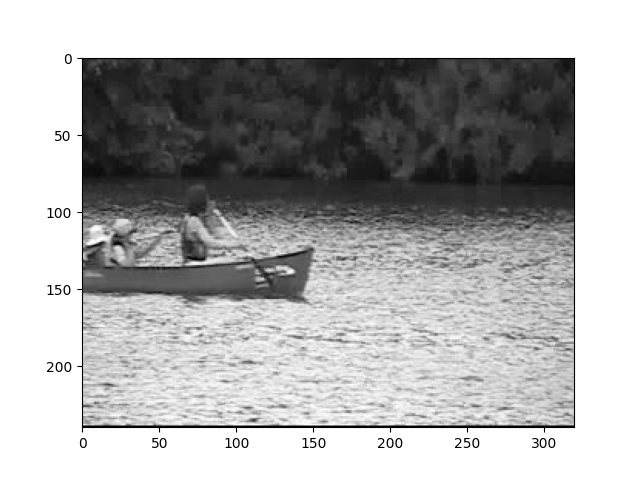
\includegraphics[width=\textwidth]{canoe_frame_100.png}
        \caption{True image}
    \end{subfigure}
    \hfill
    \begin{subfigure}{.3\textwidth}
        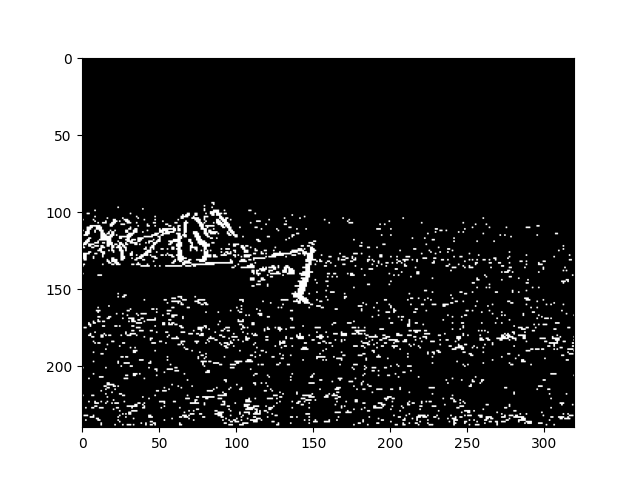
\includegraphics[width=\textwidth]{canoe_motion_frame_100.png}
        \caption{Motion mask}
    \end{subfigure}
    \hfill
    \begin{subfigure}{.3\textwidth}
        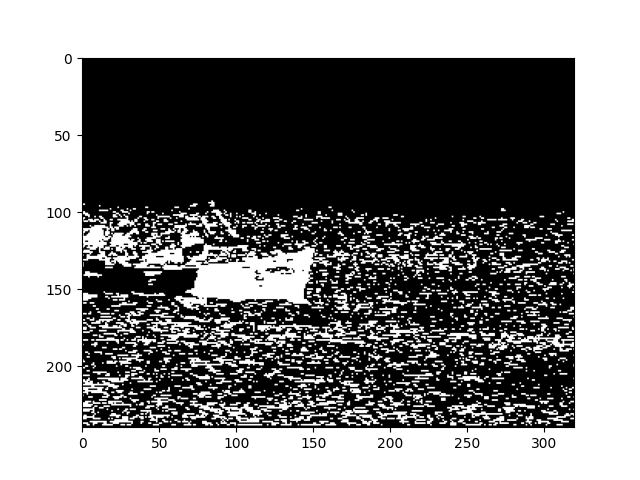
\includegraphics[width=\textwidth]{canoe_fg_frame_100.png}
        \caption{Foreground mask}
    \end{subfigure}
    \caption{Comparison of the true image, the motion mask, and the foreground mask for the canoe example at frame $100$.}\label{fig:canoe-frame-100}
\end{figure}

\subsection{Detection of Sofa}\label{subsec:sofa} % MARK: SOFA

The sofa dataset obtained from \href{changedetection.net}{changedetection.net} shows a sofa around which people move, sit down on the sofa, and handle cardboard boxes. This dataset is useful to consider because some foreground objects become part of the background, for example a box posed in front of the sofa or a person sitting down on the sofa turn into part of the localised background in the streaming DMD algorithm. This is in stark contrast to both previous examples, where the objects were clearly moving and did not stop for extended amounts of time.

This dataset does not have nearly as much noise as the canoe example from Subsection~\ref{subsec:canoe}, wherefore we choose the residual tolerances $\rho \in \set{5 \cdot 10^{-3}, 2 \cdot 10^{-3}, 1.5 \cdot 10^{-3}, 10^{-3}}$ for the corresponding memory sizes $\ell_\text{mem} \in \set{5, 10, 15, 20}$.

\begin{figure}[!ht]
    \centering
    \begin{tikzpicture}
        \pgfplotsset{
            width=16cm,
            height=7cm
        }
        \begin{axis}[
            xmin=0, xmax=100,
            ymin=4e-4, ymax=5e-1,
            ymode=log,
            xlabel={Index $i$},
            ylabel={Residual $r_i$},
            legend style={
                at={(0.975, 0.05)},
                anchor=south east,
                legend columns=1,
            }
        ]
            \addplot[color=red, smooth, thick] table[col sep=comma, header=has colnames, x index={0}, y index={1}] {sofa_motion_res.csv}; \addlegendentry{$\ell_\text{mem} = 5$}
            \addplot[color=blue, smooth, thick] table[col sep=comma, header=has colnames, x index={0}, y index={2}] {sofa_motion_res.csv}; \addlegendentry{$\ell_\text{mem} = 10$}
            \addplot[color=orange, smooth, thick] table[col sep=comma, header=has colnames, x index={0}, y index={3}] {sofa_motion_res.csv}; \addlegendentry{$\ell_\text{mem} = 15$}
            \addplot[color=black, smooth, thick] table[col sep=comma, header=has colnames, x index={0}, y index={4}] {sofa_motion_res.csv}; \addlegendentry{$\ell_\text{mem} = 20$}
        \end{axis}
    \end{tikzpicture}
    \caption{Residuals $r_i$ for the sofa dataset for memory sizes $\ell_\text{mem} \in \set{5, 10, 15, 20}$; In colour: residuals as computed during the streaming algorithm.}\label{fig:sofa-exp-residual}
\end{figure}

Similarly to the previous numerical experiments we notice that the motion mask highlights the outlines of moving foreground objects. Importantly, this example also highlights the disadvantages of the dynamic foreground detection algorithm: whenever the foreground objects come to rest the algorithm determines them to be part of the background, hence any prolonged resting may produce faulty results for the supposed foreground. A potential solution to this is to fix the dynamic background once it is established and not update it thereafter, however this also harbours the downside that the video needs to start with a stationary ``groundtruth'' background, i.e.\ the dynamic algorithm becomes subject to priming in the input data.

\begin{figure}[!ht]
    \centering
    \begin{subfigure}{.3\textwidth}
        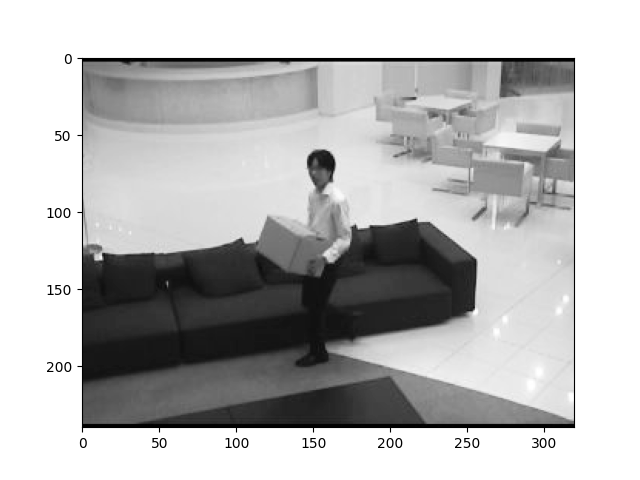
\includegraphics[width=\textwidth]{sofa_frame_100.png}
        \caption{True image}
    \end{subfigure}
    \hfill
    \begin{subfigure}{.3\textwidth}
        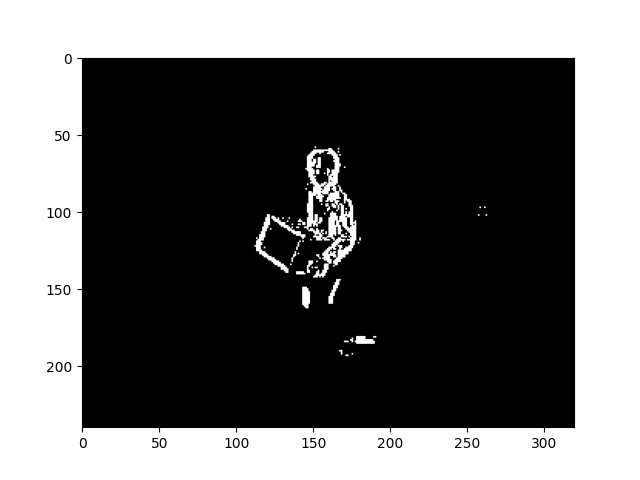
\includegraphics[width=\textwidth]{sofa_motion_frame_100.png}
        \caption{Motion mask}
    \end{subfigure}
    \hfill
    \begin{subfigure}{.3\textwidth}
        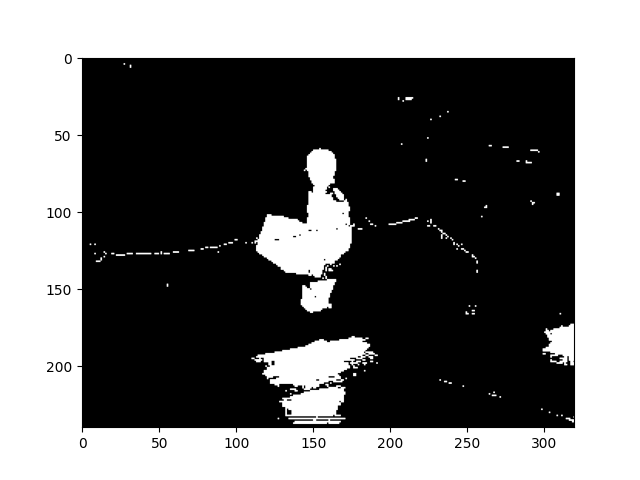
\includegraphics[width=\textwidth]{sofa_fg_frame_100.png}
        \caption{Foreground mask}
    \end{subfigure}
    \caption{Comparison of the true image, the motion mask, and the foreground mask for the sofa example at frame $100$.}\label{fig:sofa-frame-100}
\end{figure}


    \section{Conclusion and Outlook}\label{sec:conclusion}

    In this report we discuss a dynamic algorithm for motion detection and foreground/background separation in a data-agnostic setting using QR compressed streaming DMD. We demonstrate that the algorithm can produce usable and interpretable results independent of the data supplied after fine tuning of only a small number of parameters. The resulting method is significantly faster than classical DMD, where additionally all data needs to be accessible all at once. Thus, the ideas described in this report are suited in particular to real time applications, where both memory is limited and speed is of essential importance.

    To add onto the ideas of this report, a number of approaches may be eligible. Instead of applying direct QR compression one could employ a randomised method such as Randomised QR decompositions, see e.g.~\cite{Martinsson2017, Balabanov2022, Grigori2024}. Additionally, different compression regimes such as randomised DMD~\cite{Erichson2019} or compressed sensing DMD~\cite{Brunton2016a} could be used, though it would be necessary to consider if these frameworks can be efficiently adapted to a streaming framework. Furthermore, this work can be expanded by using an adaptive extension approach such as the adaptive basis update of~\cite{Hemati2014}. Another aspect to examine is the memory size --- while a fixed size snapshot memory works remarkably well, it may be that an adaptively growing or shrinking memory provides further benefits. Finally, rigorous analysis of the tolerance hyperparameters would aid in tuning the algorithm on-the-fly to avoid potentially expensive precalculations, and usage of methods to increase noise resistance would improve the performance in more challenging data settings.

    \printbibliography
\end{document}
